
\documentclass[12pt,a4paper,oneside]{article}
\usepackage[margin=1.2in]{geometry}
\usepackage{appendix}
\usepackage[dvips]{graphicx}
\usepackage{epsfig}
\usepackage{amsmath}
\usepackage{amssymb}
\usepackage{psfrag}
\usepackage[square, comma,sort,numbers]{natbib}
\usepackage{fancyhdr}
\usepackage[nottoc]{tocbibind}
\usepackage{color}
\usepackage{fixltx2e}
\usepackage{pdfpages}
\usepackage{pdflscape}
\usepackage{booktabs}
\usepackage{graphicx}
\usepackage{float}
\usepackage{afterpage}
\usepackage{subcaption}
\usepackage{lscape}
\usepackage{rotating}
\usepackage{enumitem}
\usepackage{array,tabularx}
\usepackage{fancyref}
\usepackage[dvipsnames]{xcolor}
\usepackage[colorlinks=true,allcolors=blue]{hyperref}%



\newcommand{\quotes}[1]{``#1''}

\newenvironment{conditions*}
  {\par\vspace{\abovedisplayskip}\noindent
   \tabularx{\columnwidth}{>{$}l<{$} @{\ : } >{\raggedright\arraybackslash}X}}
  {\endtabularx\par\vspace{\belowdisplayskip}}



\pagestyle{fancy}
\title{\Huge The Hat Creek Radio Observatory\\
\vspace{0.5cm}
The IF Splitter\\
\vspace{0.5cm}
\normalsize \emph{}
\vspace{3.5cm}
\begin{center}

\includegraphics[height=4cm]{titlepage/SETI_institute_logo.jpg}
\end{center}
}
\author{ 
\vspace{1cm}
\Large
\textbf{ Alexander Pollak \& Marc Jacquart} \\
SETI Institute \\ 
189 Bernardo Ave, Suite 200 \\
Mountain View, CA 94043 \\ 
Alexander.Pollak.87@gmail.com\\
}
\date{\today}



\begin{document}
\clearpage\maketitle
\thispagestyle{empty}

%\newpage
%\thispagestyle{empty}
%\section*{Abstract}
%\noindent 
%



%
%\vspace{3cm}
%\begin{flushright}
%Alexander Pollak \\ \emph{September, 2015}
%\end{flushright}

%\newpage
%\thispagestyle{empty}
%\tableofcontents
\newpage

%----------------------------------------------------------------------------------------
%	General
%----------------------------------------------------------------------------------------
%\pagestyle{plain}
\section{General}
\label{sec:General}
% ----------------------------------------------------------------

This document outlines general information regarding the IF Splitter such as the design, parts, wiring, cabling, and testing. This information is aimed at detailing the entire process of creating an IF Splitter from design to manufacturing to testing. 


%----------------------------------------------------------------------------------------
%	CAD Design and Drawings
%--------------------------------------------------------------------------------------

\section{CAD Design and Drawings}
\label{sec:CAD}
% ----------------------------------------------------------------
This section includes a description of the CAD design. Figure \ref{fig:CAD_outside} shows the outside of the IF splitter with the front pannel. Figure \ref{fig:CAD_inside} shows the IF splitter open, with the mounts and signal splitter modules but no cable. The par list is available in appendix \ref{sec:Part_List}. The Drawings are available in appendix \ref{sec:Drawings}.

\hfill \break

%
\begin{figure}[H]
\centering
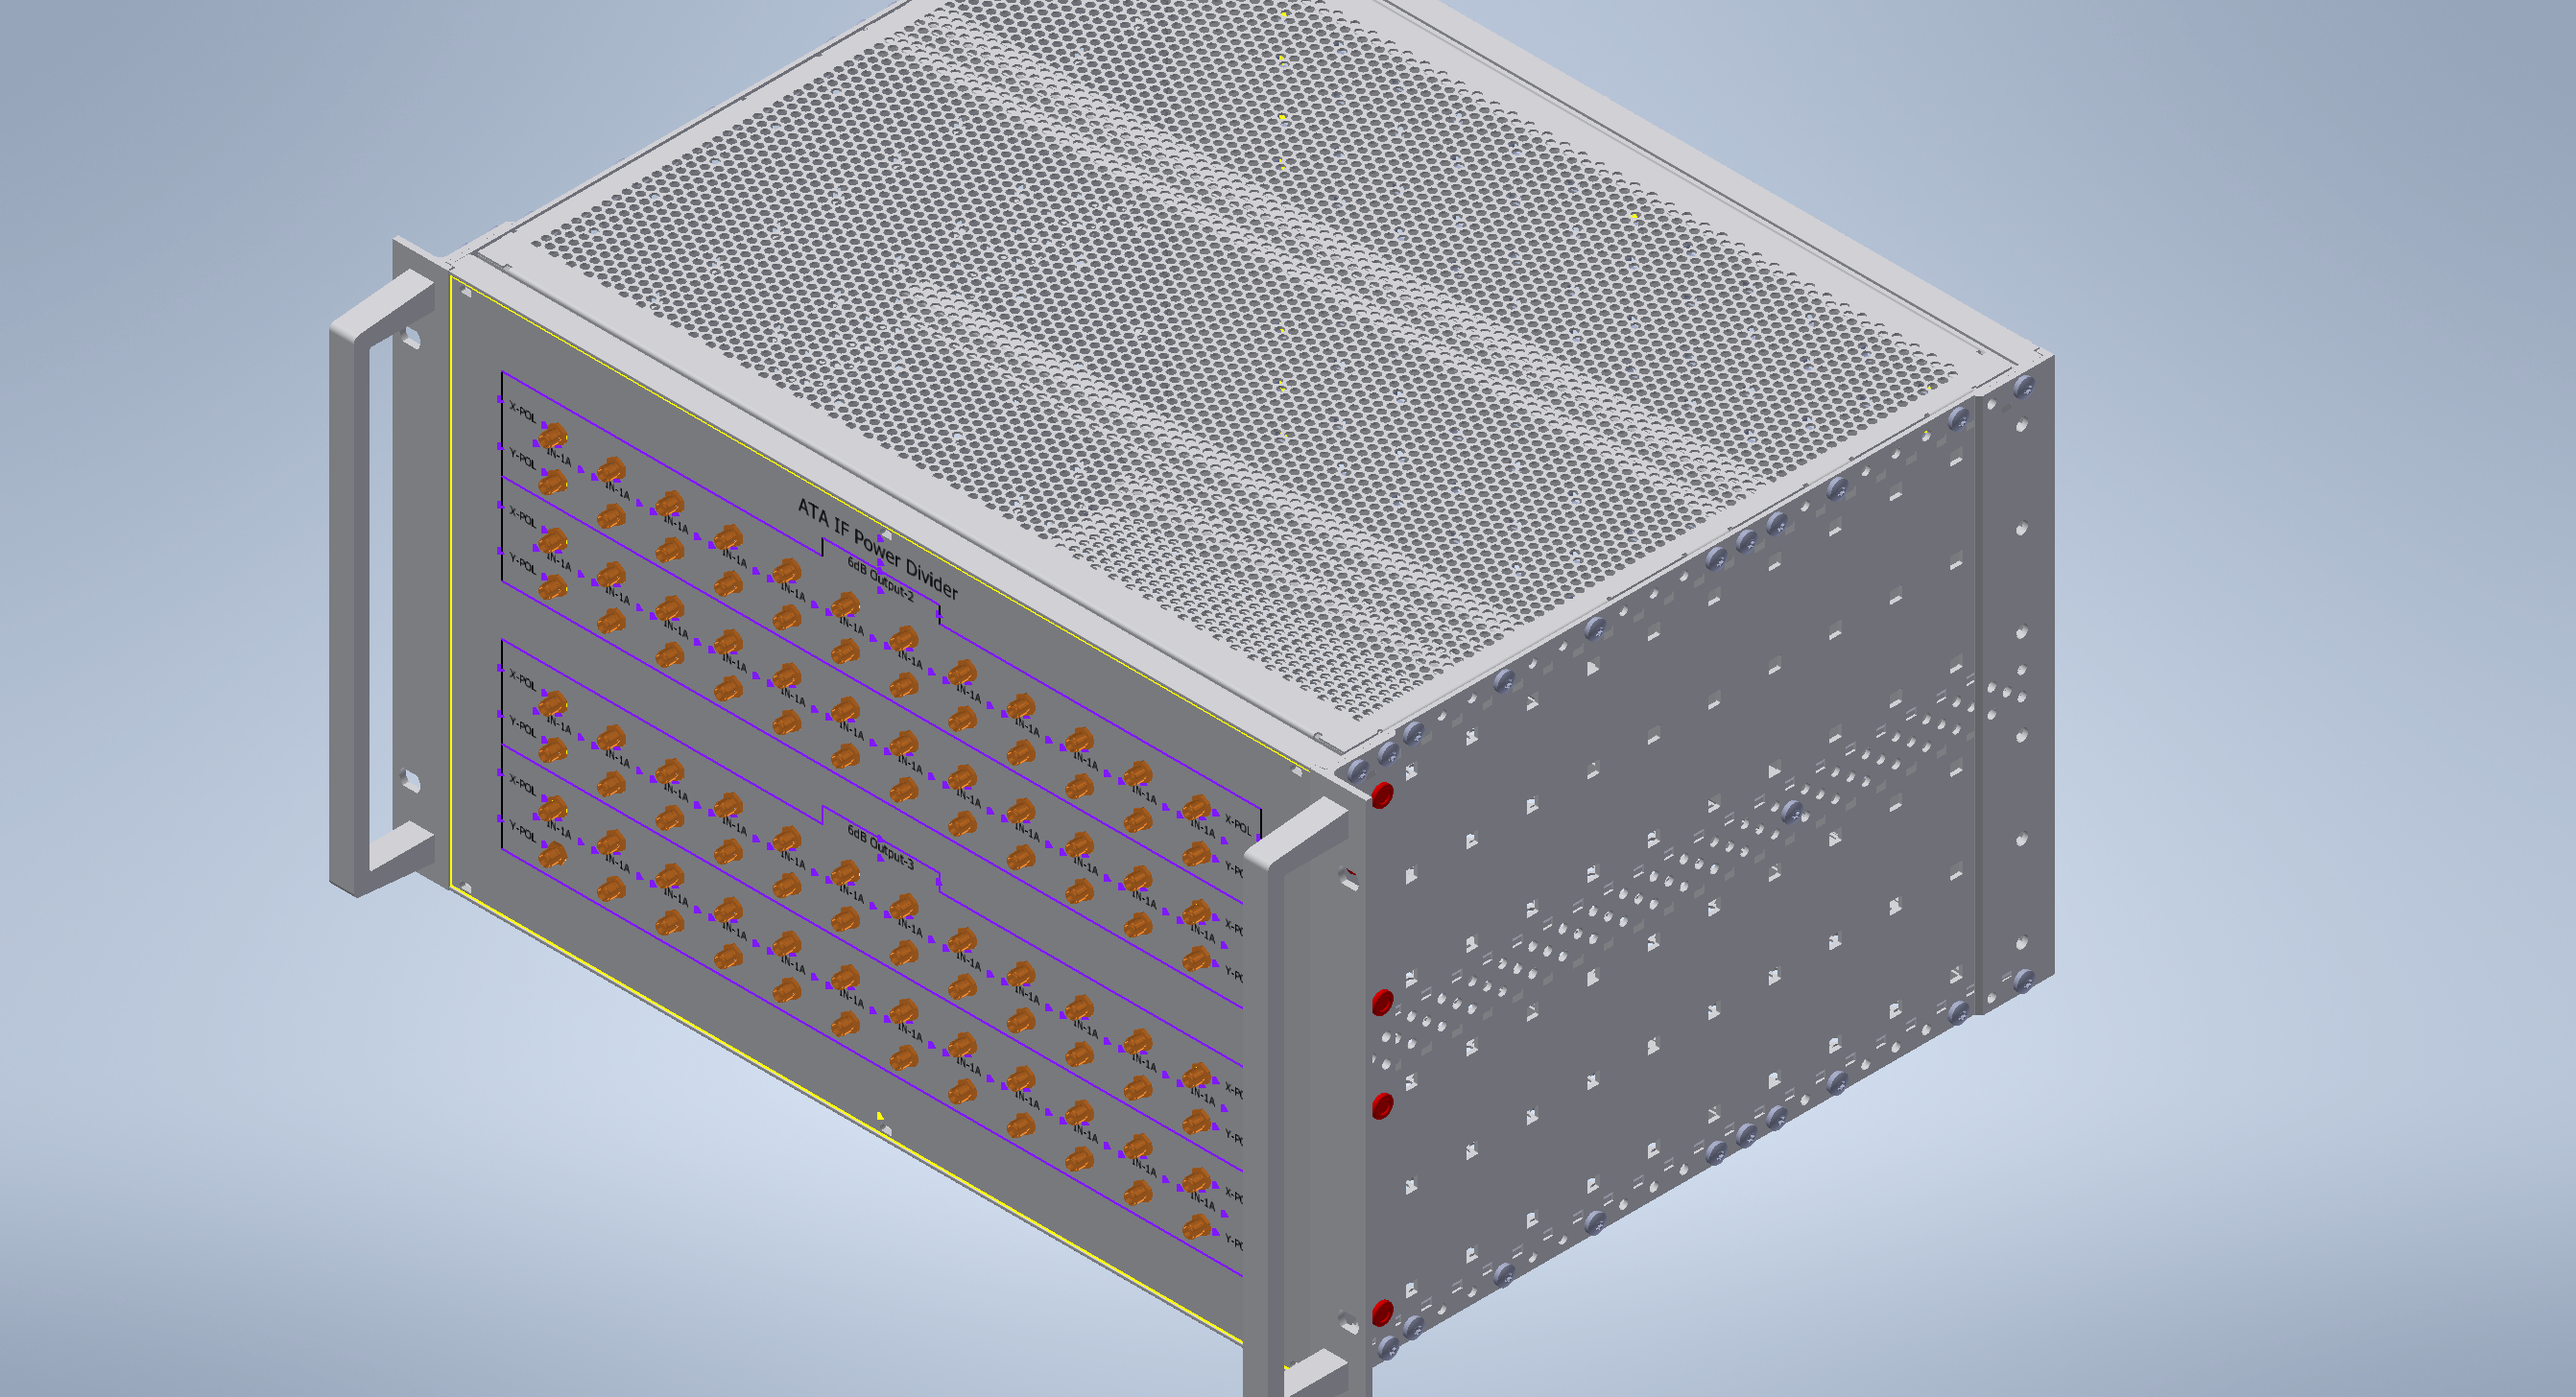
\includegraphics[width=1\linewidth]{figures/CAD_outside.png}
\caption{Outside CAD view of the IF splitter.}
\label{fig:CAD_outside}
\end{figure}
%

%
\begin{figure}[H]
\centering
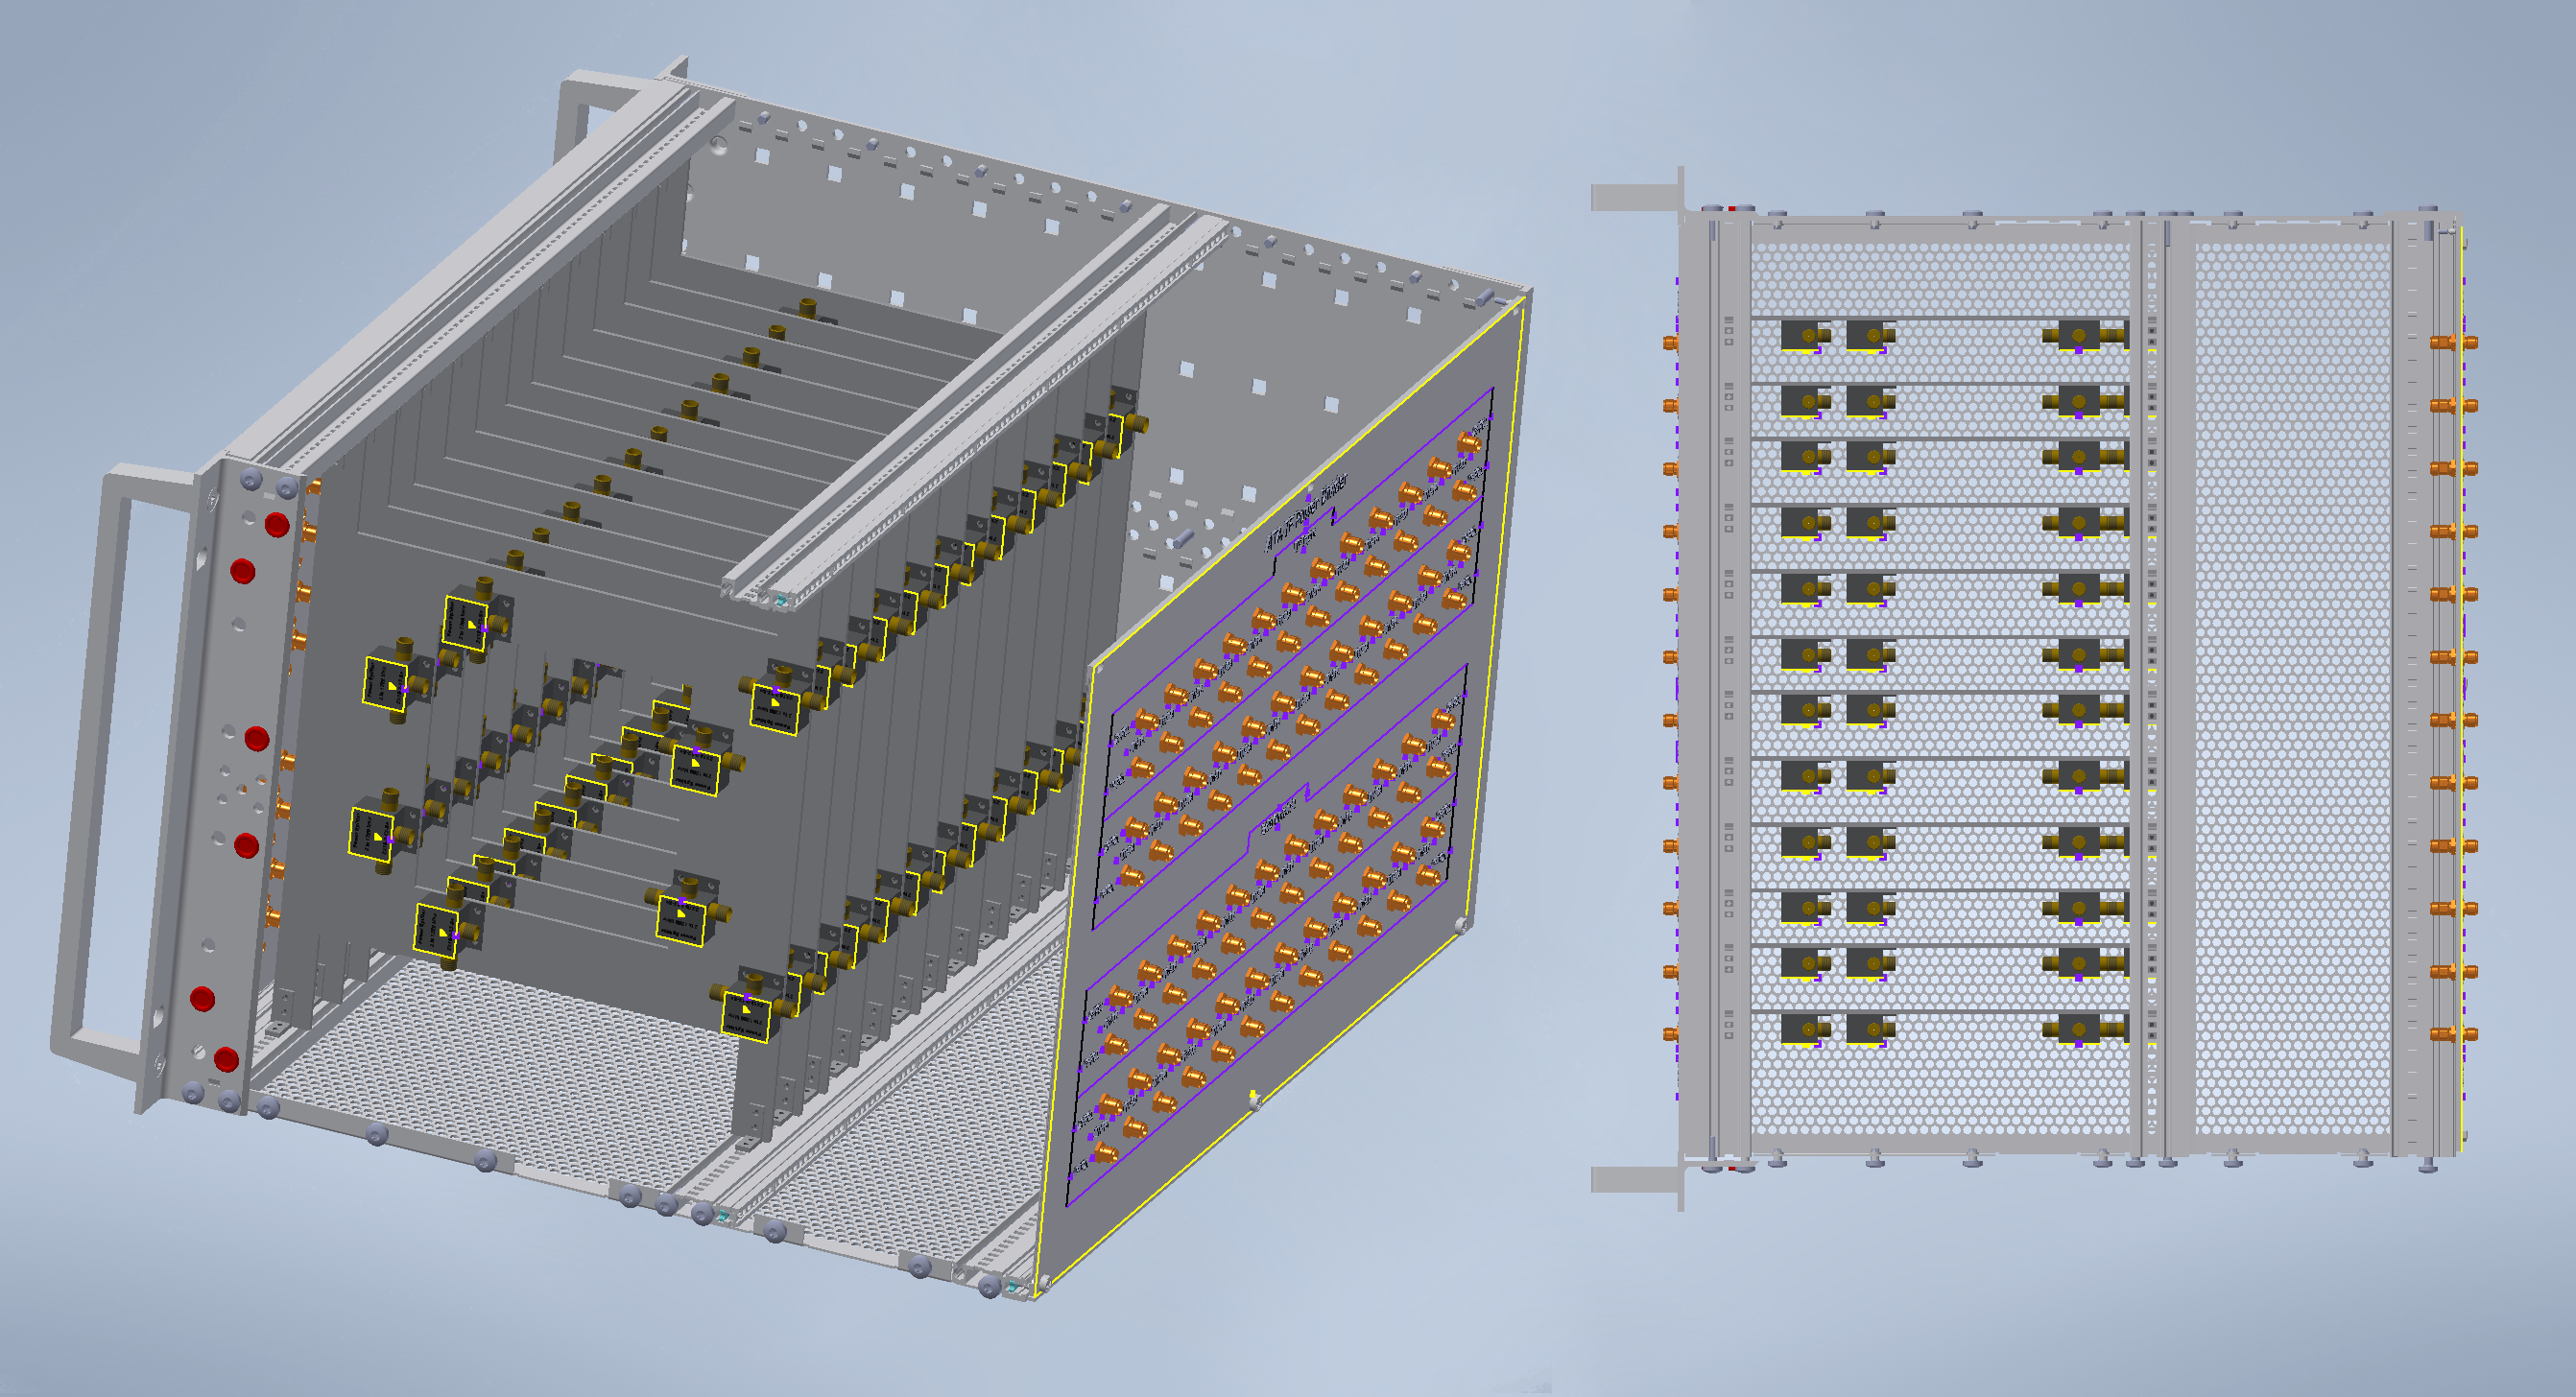
\includegraphics[width=1\linewidth]{figures/CAD_inside.png}
\caption{Inside CAD view of the IF splitter.}
\label{fig:CAD_inside}
\end{figure}
%


\subsection{Design}
\label{sec:Design}
% ----------------------------------------------------------------


%--
\subsection{Wiring}
\label{sec:Wiring}
% ----------------------------------------------------------------


\subsection{Testing}
\label{sec:Testing}
% ----------------------------------------------------------------

%----------------------------------------------------------------------------------------
%	Power Supplies & Adapter
%----------------------------------------------------------------------------------------
\section{Power Supplies \& Adapter}
\label{sec:Power}
% ----------------------------------------------------------------
All the components in the IF splitter are passive and don't require any power supply.
%----------------------------------------------------------------------------------------
%	Module Wiring
%--------------------------------------------------------------------------------------


\subsection{Front Panel}      
\label{sec:FrontPannel}
% ----------------------------------------------------------------

%----------------------------------------------------------------------------------------
%	Module Testing
%----------------------------------------------------------------------------------------
\section{Testing}
\label{sec:Testing}
% ----------------------------------------------------------------


\subsection{Setup}
\label{sec:Testing_Setup}
% ----------------------------------------------------------------


\subsection{Method \& Desired Results}
\label{sec:Testing_Method}
% ----------------------------------------------------------------

\subsection{Troubleshooting}
\label{sec:Testing_Troubleshooting}
% ----------------------------------------------------------------

\newpage
 
%----------------------------------------------------------------------------------------
%	Appendix: Attemplifier Module Enclosure Drawings
%----------------------------------------------------------------------------------------

\appendix
% ----------------------------------------------------------------

% To include pages from other PDFs
% 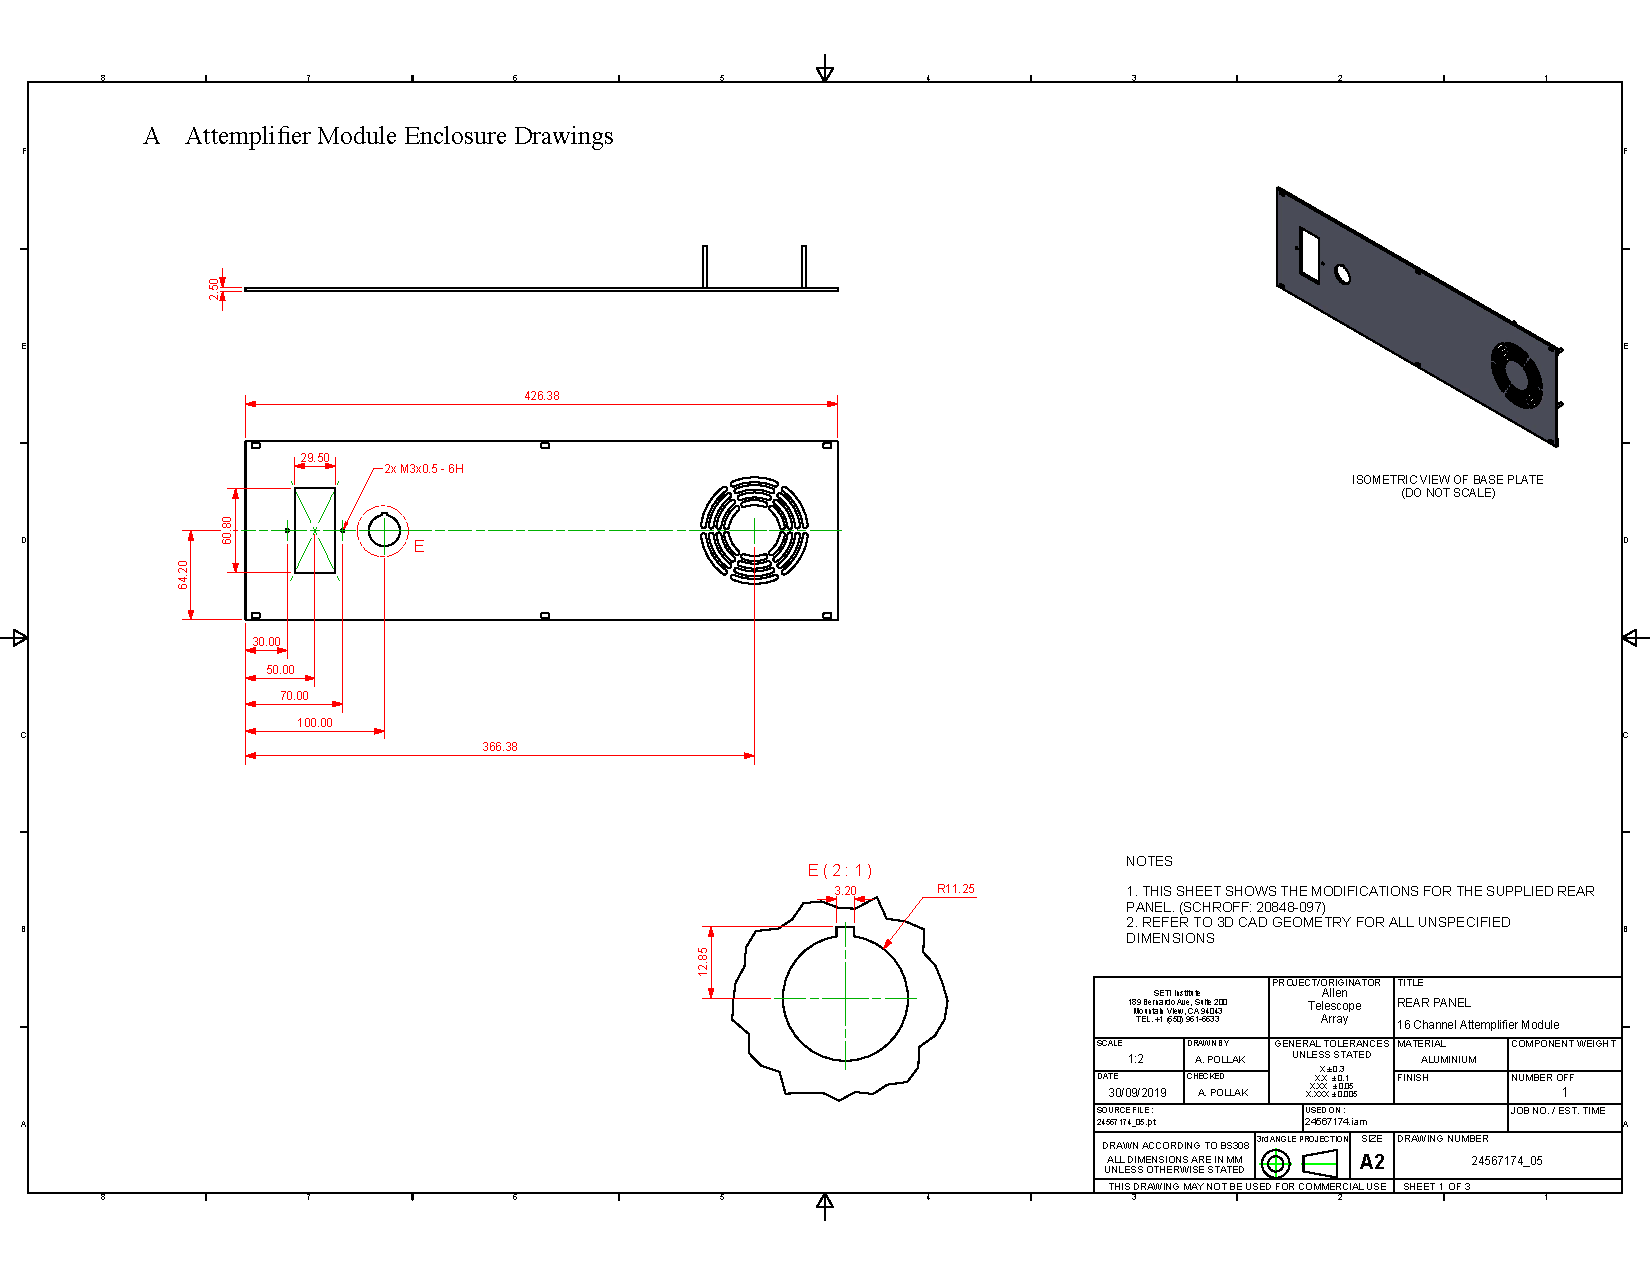
\includepdf[pages=-, landscape=true]{Documentation/PDFs/24567174_05(copy).pdf}


%----------------------------------------------------------------------------------------
%	Appendix: IF splitter Component List
%----------------------------------------------------------------------------------------
\begin{landscape}
\section{Component List of IF Splitter}\label{sec:Part_List}

% ----------------------------------------------------------------

\begin{table}[H]
\centering
\resizebox{1.5\textwidth}{!}{%
\begin{tabular}{@{}lllllll@{}}
\toprule
Qty & Unit & Description & Manufacturer & PN Manufacturer & Distributor & PN Distributor\\
\midrule
12 & Each & Power Splitter Mount & & &\\
96 & Power Splitter module & & &\\
336 & each & Screws (type?) & & &\\
% 12 * 12 = 144 for L-brackets
% 16 * 12 = 192 to attach power splitter modules on mount
%

\bottomrule            
\end{tabular}}
\label{tab:IF_components}
\end{table}

%----------------------------------------------------------------------------------------
%	Appendix: Control Board Schematics
%----------------------------------------------------------------------------------------

\section{Drawings}
\label{sec:Drawings}
Below are the drawings of the front pannel, Power Splitter Mount and L-shape attachement brackets.
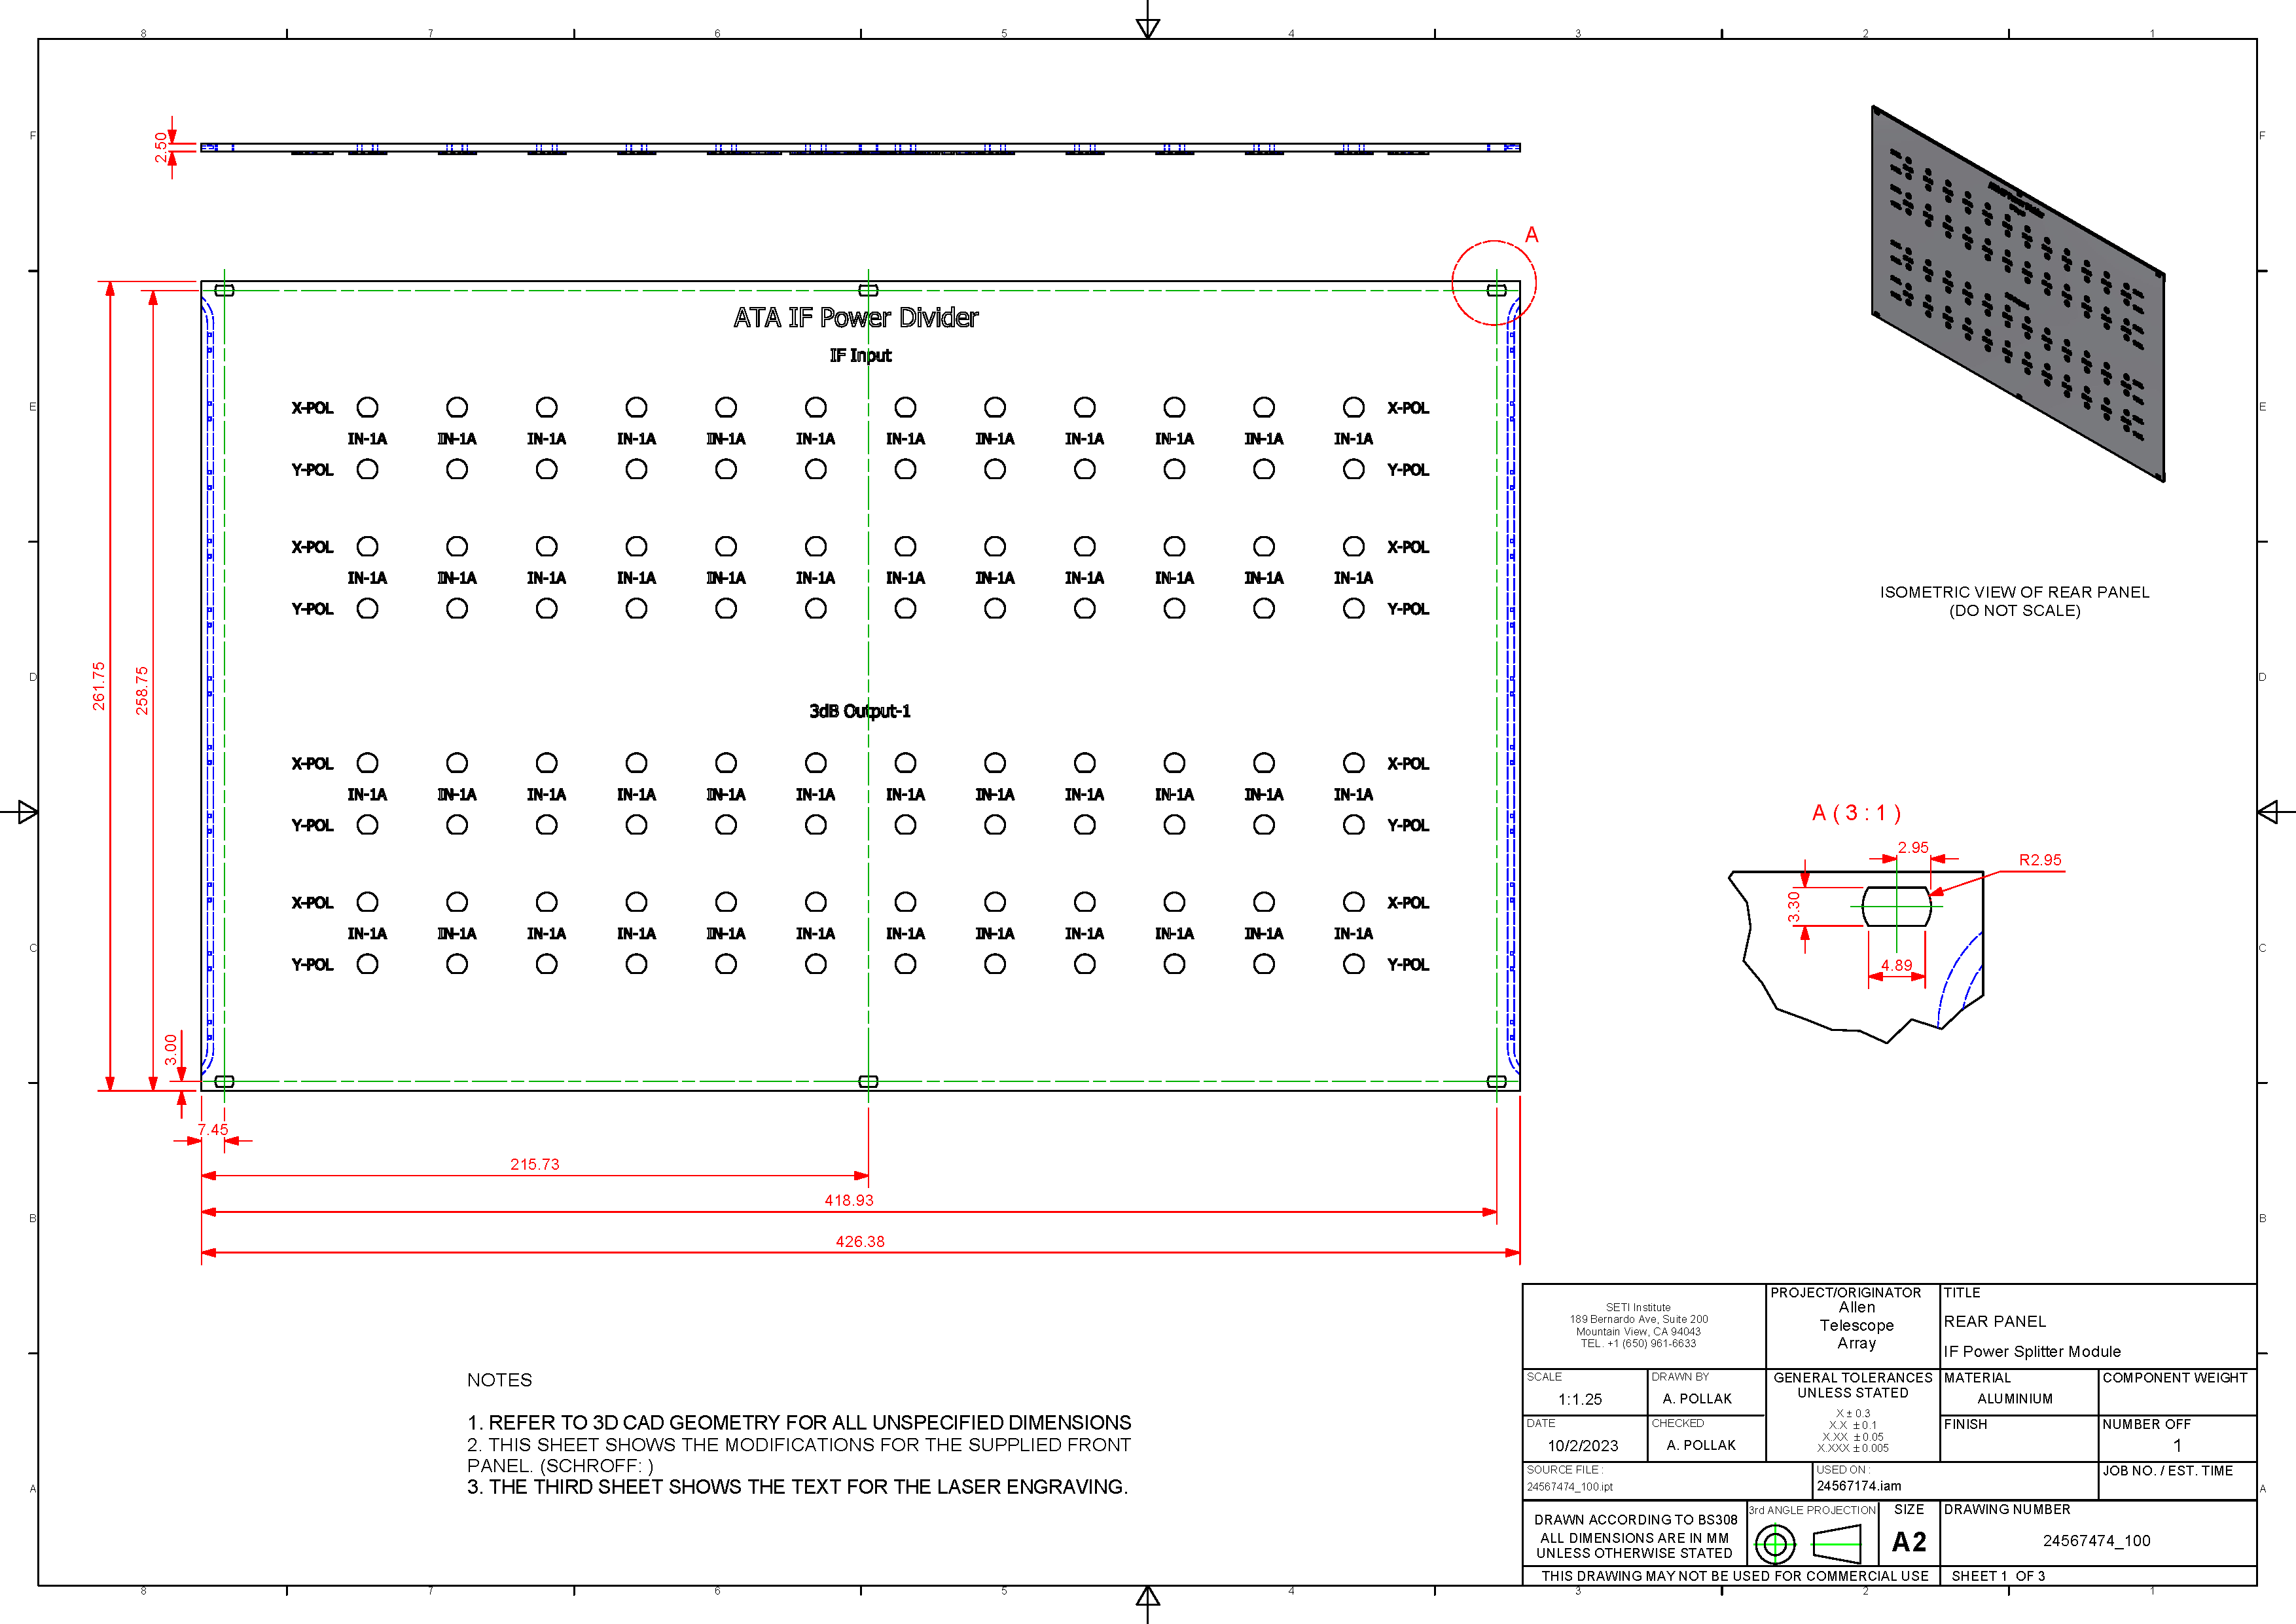
\includepdf[pages=1-2, landscape=true]{PDFs/24567474_100.pdf}
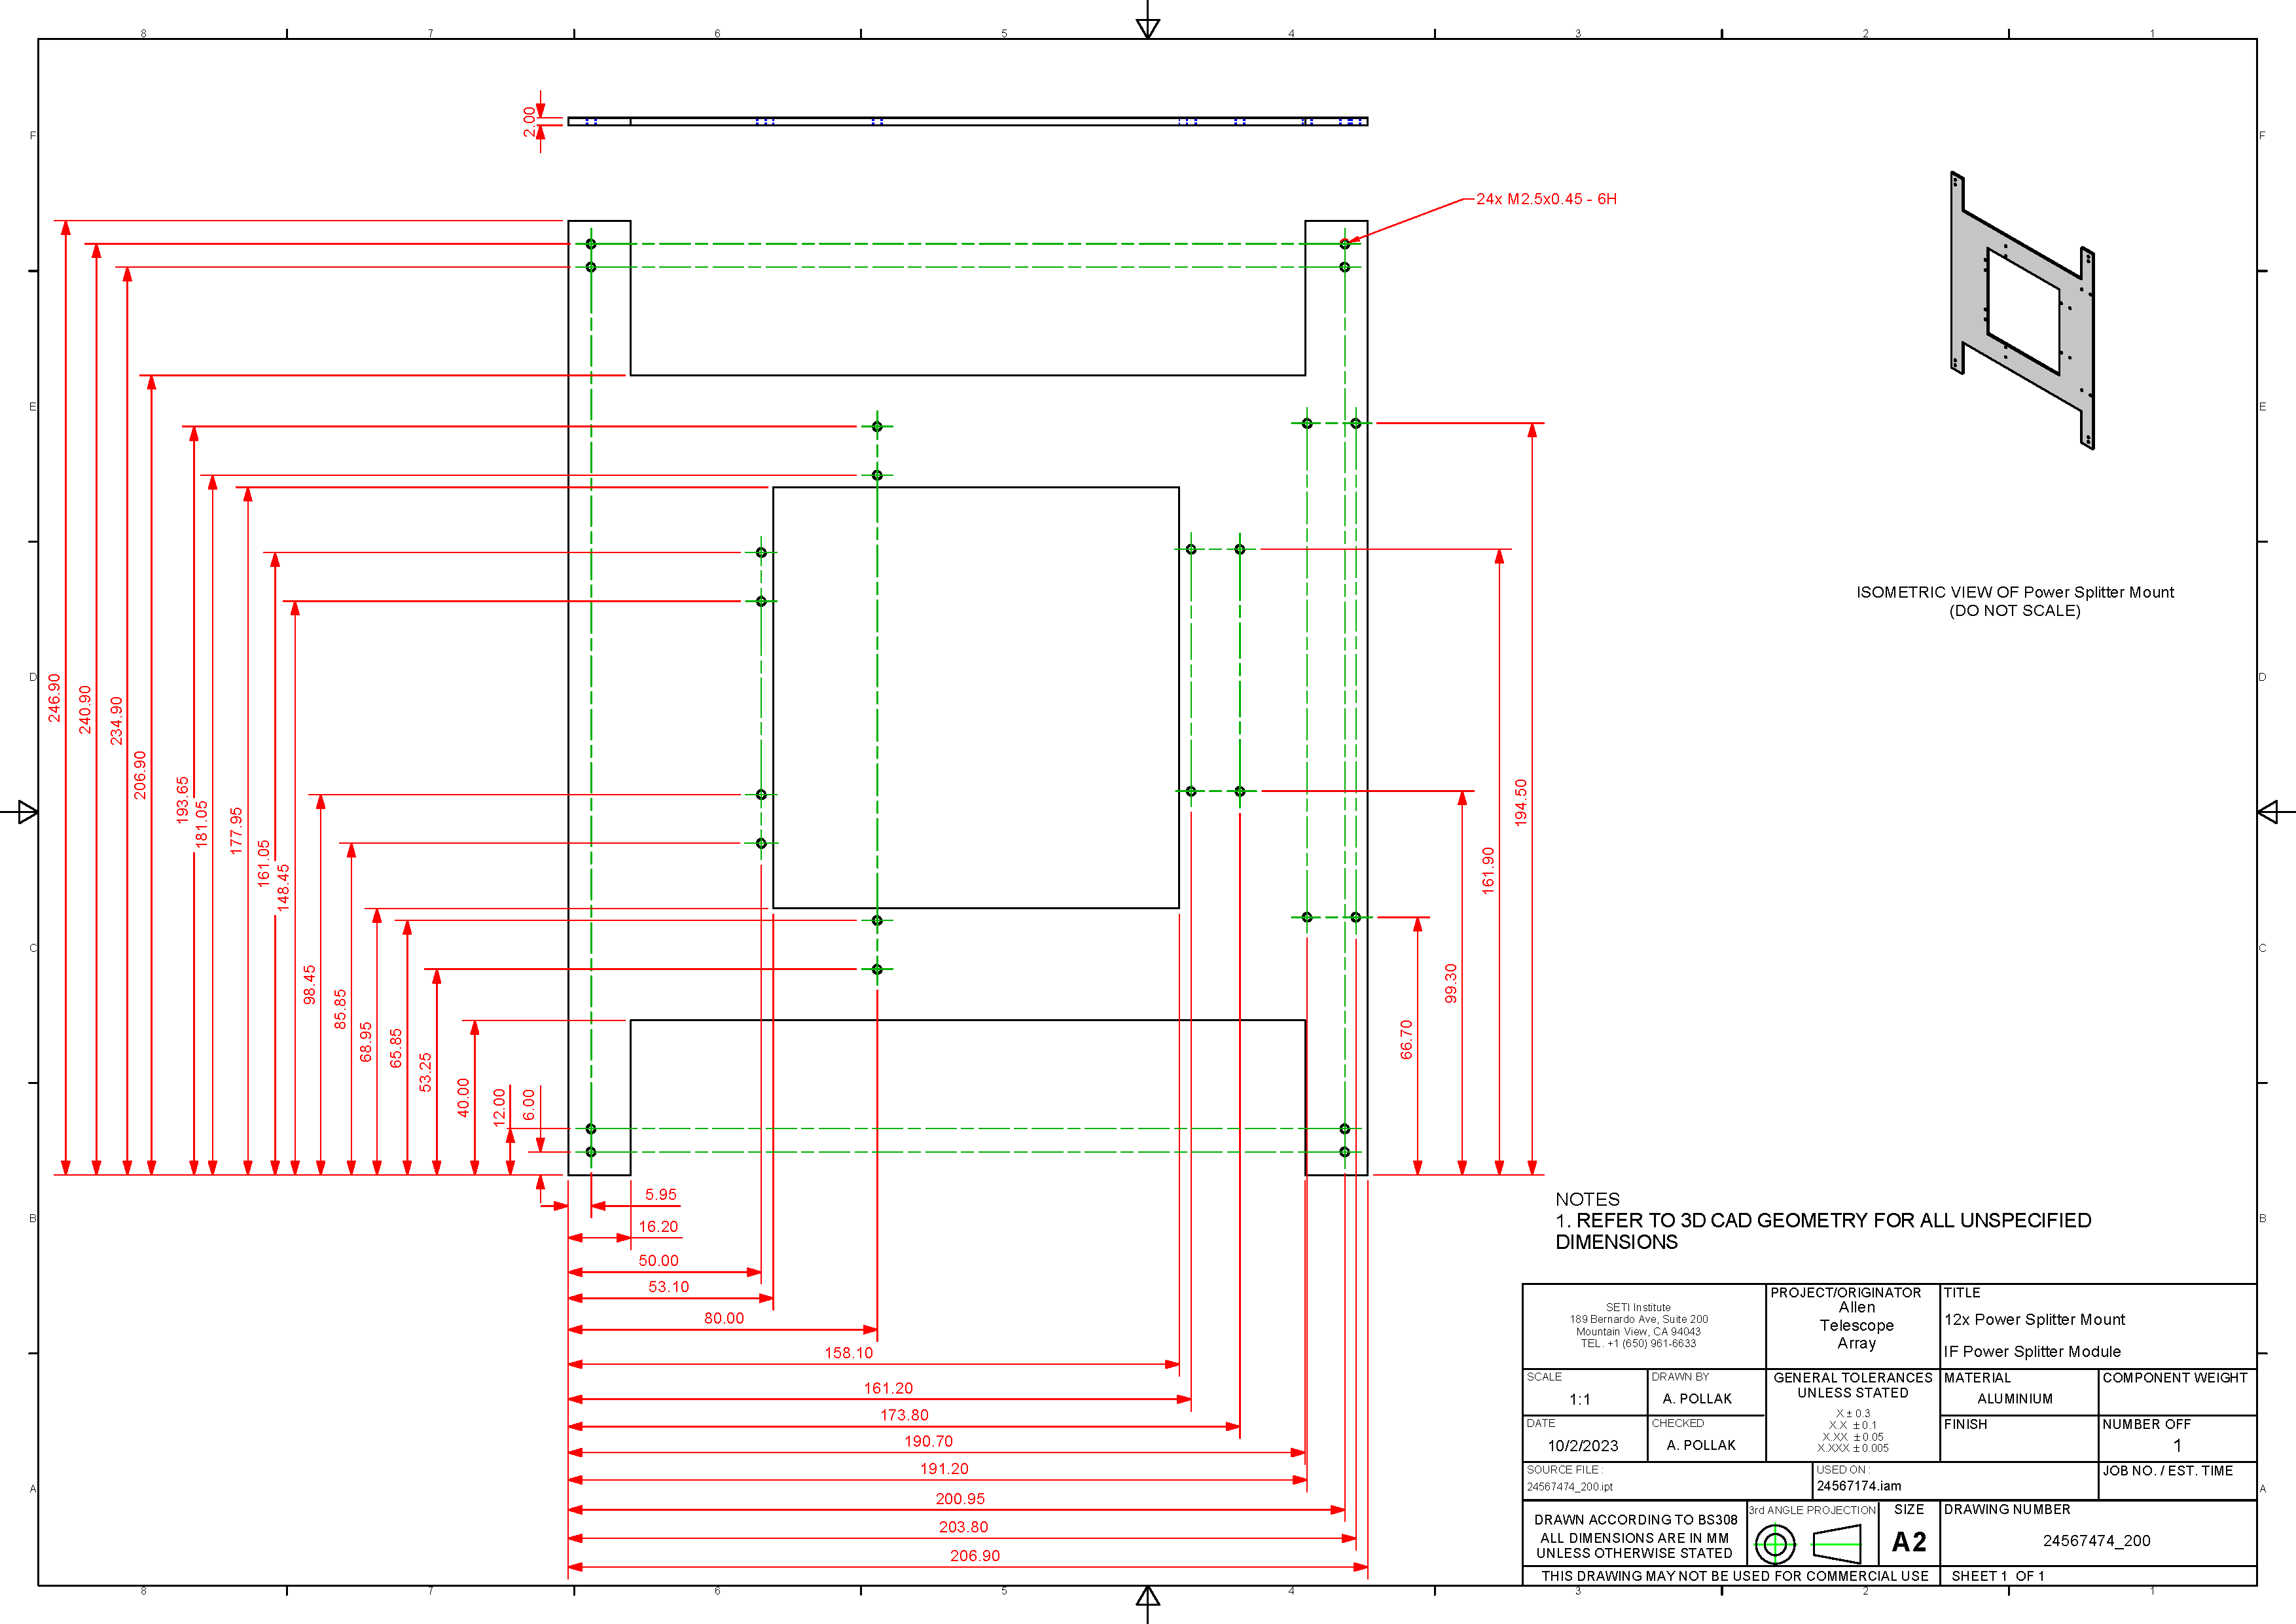
\includepdf[pages=-, landscape=true]{PDFs/24567474_200.pdf}
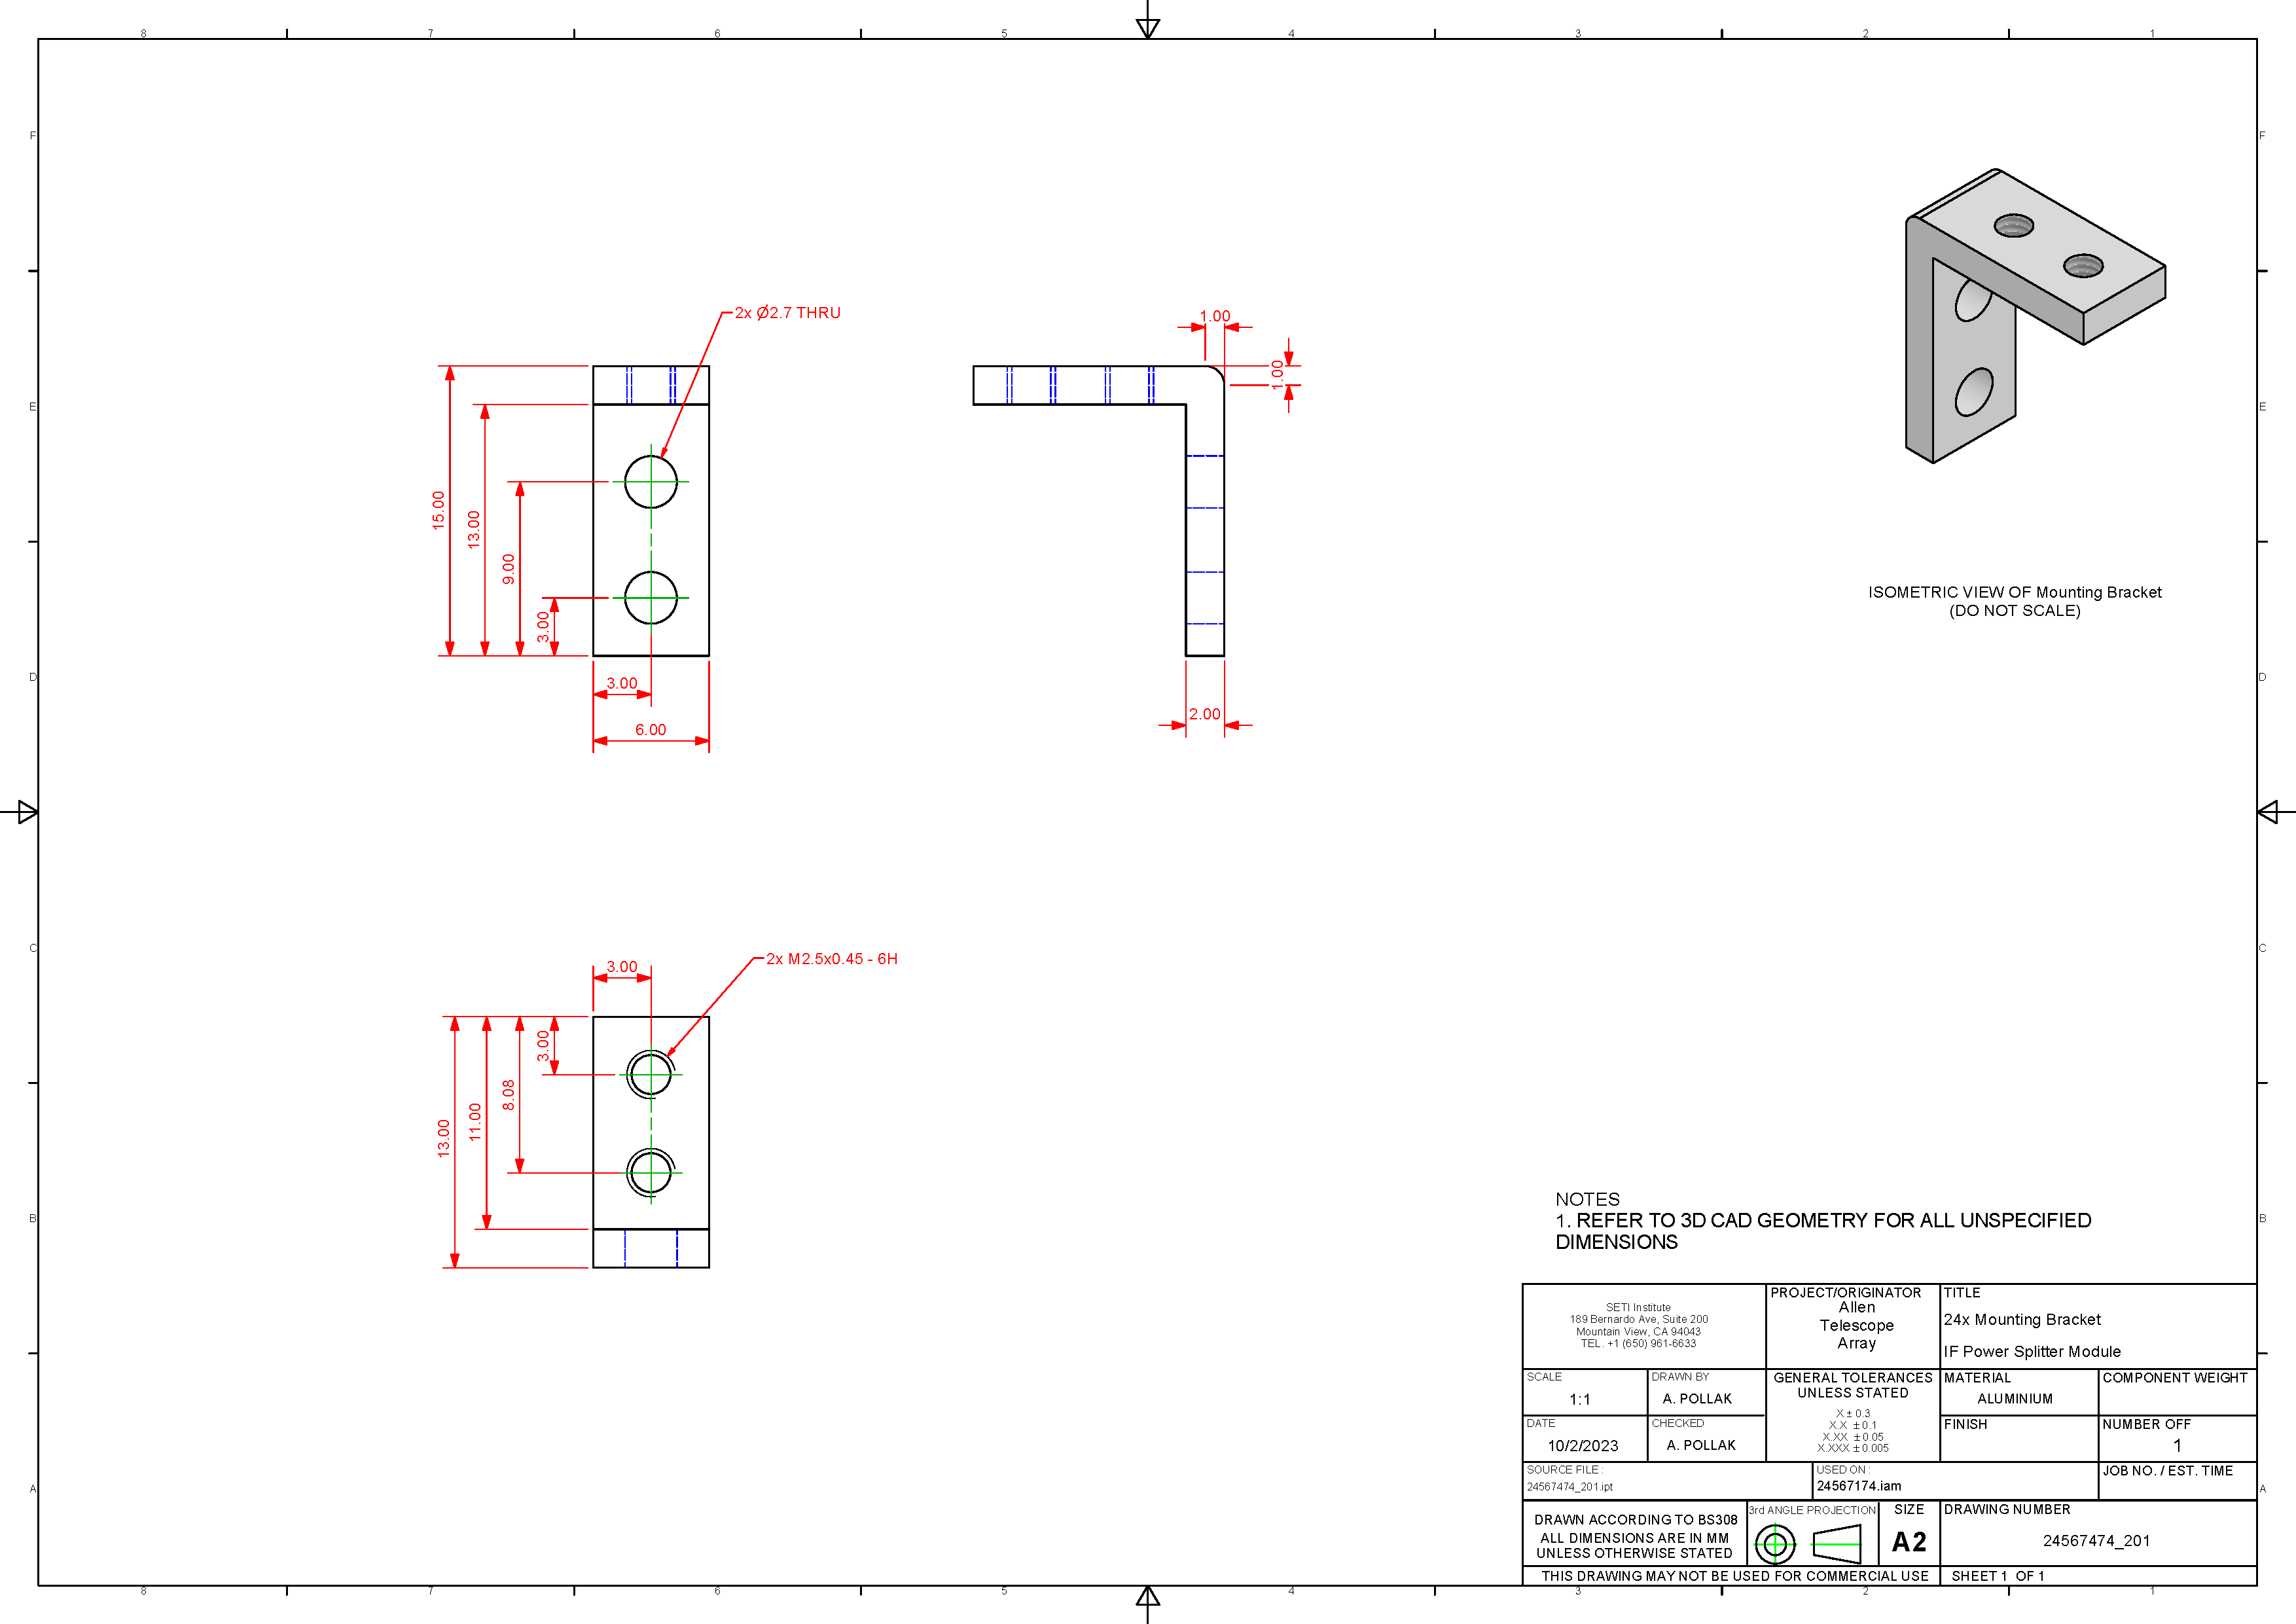
\includepdf[pages=-, landscape=true]{PDFs/24567474_201.pdf}
% ----------------------------------------------------------------

%
%\begin{figure}[H]
%\centering
%\includegraphics[width=1\linewidth]{<path>/picture.png}
%\caption{Caption}
%\label{fig:LABEL}
%\end{figure}
%

\end{landscape}

%----------------------------------------------------------------------------------------
%	Appendix E: Attemplifier Enclosure Drawings
%----------------------------------------------------------------------------------------
\begin{landscape}
\section*{E \hspace{.5cm} Attemplifier Enclosure Drawings}

% ----------------------------------------------------------------

%
%\begin{figure}[H]
%\centering
%\includegraphics[width=1\linewidth]{<path>/picture.png}
%\caption{Caption}
%\label{fig:LABEL}
%\end{figure}
%
\end{landscape}
\end{document}
